% Font must be at least 12pt, 10pt for figures
\documentclass[12pt, letterpaper]{article}


\usepackage{cosyne_abstract}
\usepackage{siunitx}

\usepackage{etoolbox}
\bibliographystyle{cosyne_abstract}
\pagenumbering{gobble}

\newcommand{\subrefb}[1]{(\subref{#1})}



\date{}
\author{}
% Enter paper title to populate PDF metadata:
\hypersetup{pdftitle={Ring attractors for three-dimensional navigation in bats}}
\makeatletter

% Enter path to PDF file with figures:

% Enter title:
\title{\color{custom}\large{\vspace{-1.5cm}%
Ring attractors for three-dimensional navigation in bats}}


\begin{document}

\maketitle
\vspace*{-2cm}

\textbf{Summary:} Head direction (HD) cells in rats are well described by one-dimensional attractor networks~\cite{Taube1990,Zhang1996}, in which a localized activity bump encodes the animal's heading. This framework is insufficient for animals that navigate freely in three dimensions, such as bats. HD cells recorded in bats are organized in toroidal coordinates~\cite{Finkelstein2015}: some are tuned to a single angle (yaw or pitch), others to conjunctions of angles. A unified computational account of these observations is still lacking.

Here, we present minimal attractor-network models of the bat HD system that reproduce these firing patterns and cell types. The models combine two ring attractors, each integrating a different component of the vestibular input. Conjunctive HD cells functionally couple the resulting one-dimensional vestibular representations to a two-dimensional visual representation, which allows sparse visual information to correct the noise-induced drift of the attractor state.

To derive experimentally testable predictions, we compare two architectures for coupling the HD system to visual input: landmark information is associated either with a conjunctive layer or directly with the ring neurons. We characterize their distinct dynamics; in both, Hebbian plasticity learns the visual--HD connectivity, offering a possible mechanism for associating visual features with head direction.

Our framework is a starting point for more extensive modelling of the bat HD system. Three-dimensional navigation introduces additional degrees of freedom that cannot be captured by simply extending one-dimensional models. The problem is not specific to bats: recent recordings suggest that rodent HD cells also update their reference frame during three-dimensional movement~\cite{Williams2026}, but its relation to the tuning reported in bats~\cite{Finkelstein2015} remains an open question. By capturing key experimental features in a minimal model, our work provides a basis for addressing such questions and motivates further modelling and experiments on three-dimensional HD coding and its interaction with the visual system.


\vspace*{-0.2cm}
\hrulefill

\textbf{Additional Details:} Our model uses rate-based neurons, with recurrent connectivity within each ring attractor as described in~\cite{Zhang1996}. Vestibular angular-velocity signals with respect to the yaw and pitch axes modulate the gain of the corresponding ring, thus integrating head movements in 3D. Additive Gaussian noise, implemented as a Wiener process, emulates neural variability. 

We explore two network configurations for conveying sensory feedback to the ring attractors. Sparse visual feedback is either projected from 3D landmark cells to a conjunctive cell layer that represents the full toroidal space, or projected directly to the yaw/pitch rings (\Cref{subfig:conj_feeback,subfig:direct_feedback}). Both employ dynamic weights based on normalized Hebbian learning~\cite{Miller1994} to learn the association between landmark cells and the HD system. Landmark cells have Gaussian tuning curves and become active when a landmark enters the bat’s visual field. In both models, conjunctive cells sum feedforward input from both rings and are thresholded by a negative bias. The models differ in the role of the conjunctive population: in the first model, the conjunctive cells mediate feedback but can also be thought of as representing a specific conjunction of pose and current visual input. In the direct feedback model, conjunctive cells could be sparser (need not cover all visual feedback instances) and thought of as encoding, e.g., poses of interest (e.g., for association with place fields downstream).

Both models replicate the main HD cell types observed in flying bats~\cite{Finkelstein2015}. The trial-averaged firing rates of one representative cell per tuning pattern are shown in \Cref{subfig:cell_types}. Notably, yaw-tuned cells shift their azimuth tuning by \ang{180} upon inversion (\Cref{subfig:inversion}), which was a key feature of the toroidal coordinate encoding observed in~\cite{Finkelstein2015}. \Cref{subfig:drift_comparison} shows the average error over repeated trials for both mechanisms. While both provide stable anchoring, their firing rates differ markedly when visual feedback is absent (i.e. in the dark \Cref{subfig:darkness_fire_rate}), thus suggesting experiments to disambiguate the models.

We tested the models by simulating bat flights in an enclosed environment. Speed was modelled as an Ornstein--Uhlenbeck process~\cite{Gillespie1996}, with an additional slowdown near the wall. Heading followed the same type of process, with an added turn away from the wall that scales linearly with wall proximity. A similar repulsion prevented unrealistic upward- or downward-facing flights. An example of such a generated flight pattern is displayed in \Cref{subfig:trajectory}. Roll was not simulated, as roll-sensitive cells are sparse~\cite{Finkelstein2015} and have not been characterized in detail. Their interplay with yaw and pitch is nevertheless likely relevant for a consistent three-dimensional code and warrants further experiments.

Finally, we tested a single toroidal attractor, as proposed in~\cite{McNaughton2006} and observed for grid cells in~\cite{Gardner2022}. This architecture performed worse, required far more neurons than two rings, and nevertheless showed stronger drift (\Cref{subfig:torus_comparison}). It would also not predict the cells tuned exclusively to yaw or pitch reported in~\cite{Finkelstein2015}, which the two-ring architecture accounts for naturally.


\begin{figure}[!b]
    \centering
    \hspace{0.01\textwidth}
    \begin{subfigure}{0.3\textwidth}
        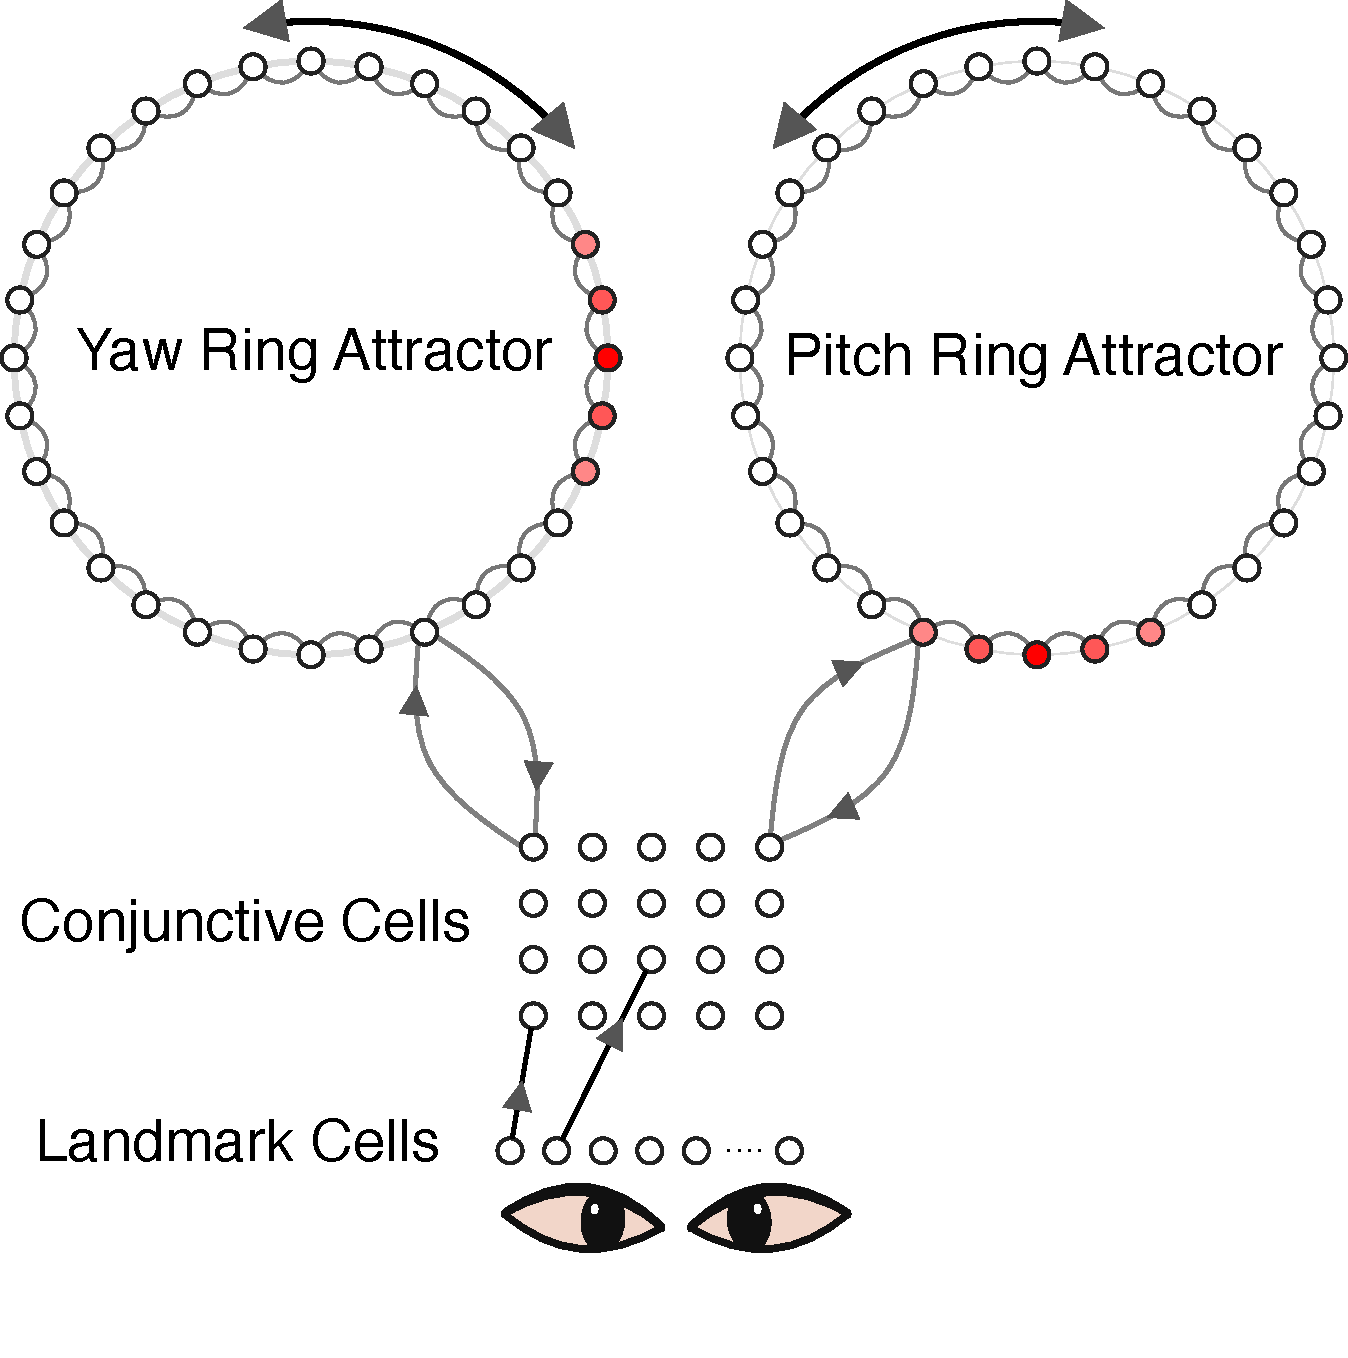
\includegraphics[width=1.0\textwidth]{figures/bat_hd_conj_feedback.pdf}
        \caption{}
        \label{subfig:conj_feeback}
    \end{subfigure}
    \hspace{0.02\textwidth}
    \begin{subfigure}{0.3\textwidth}
        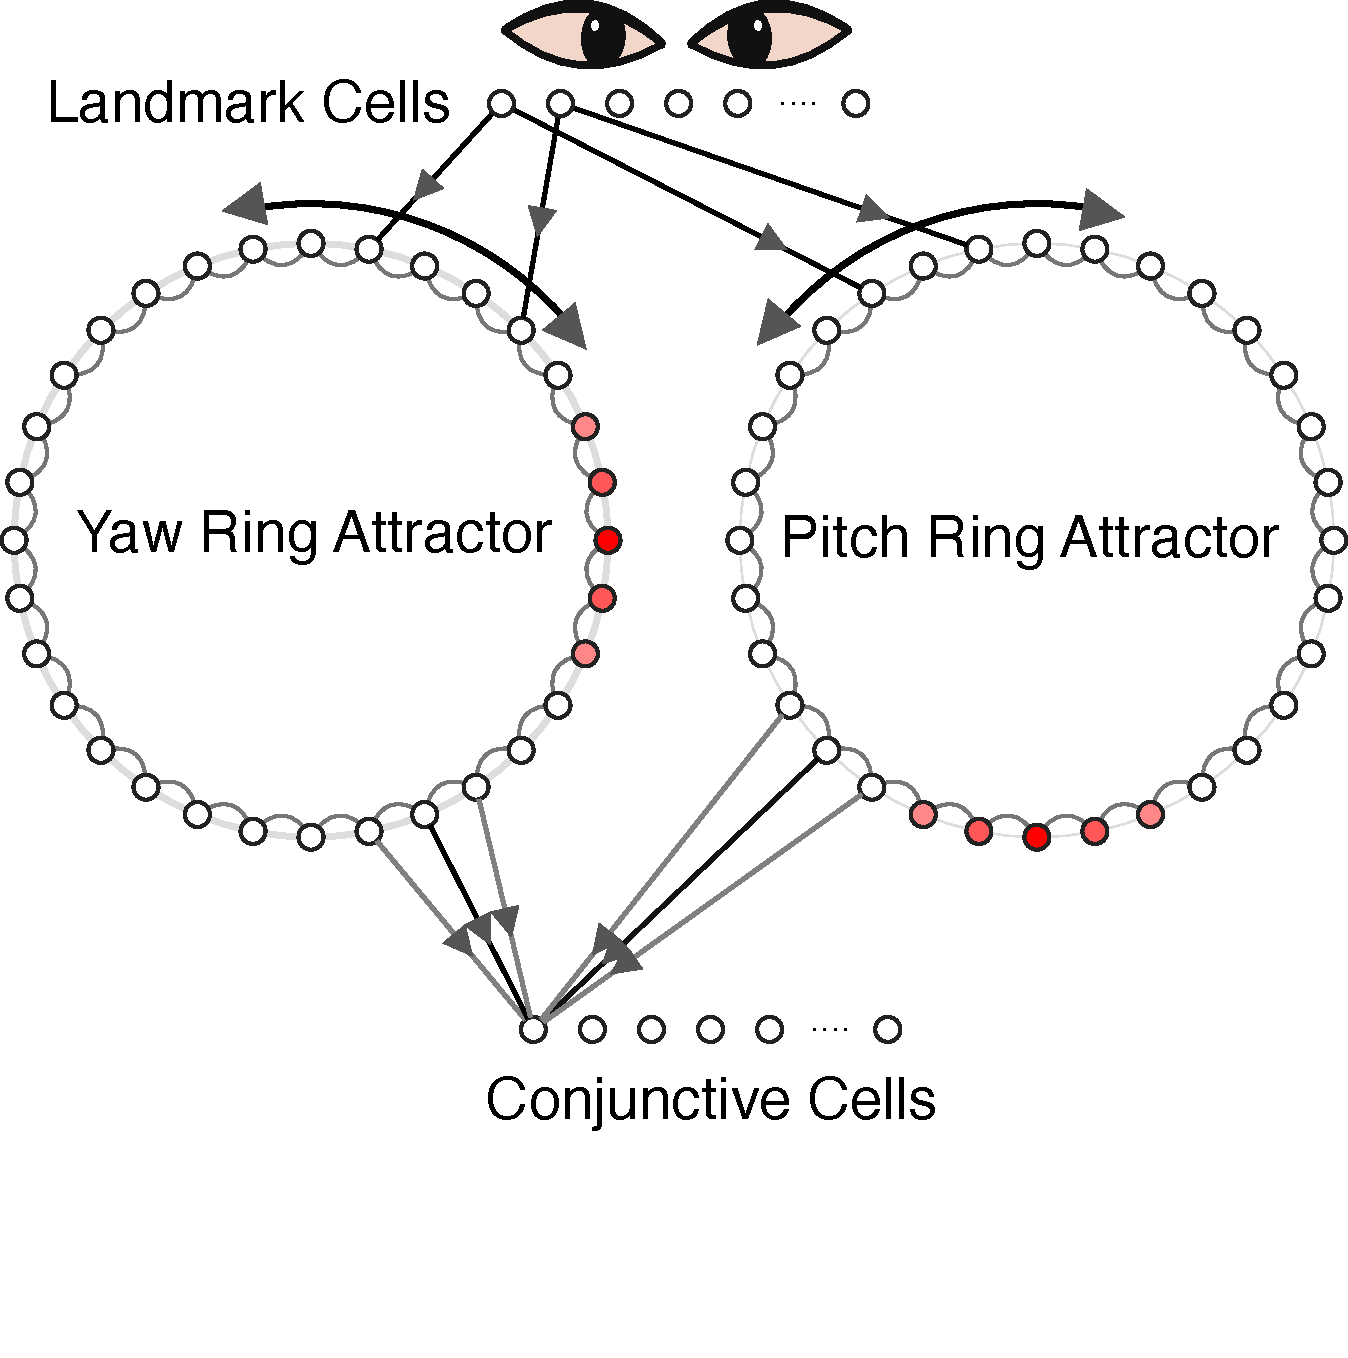
\includegraphics[width=1.0\textwidth]{figures/bat_hd_direct_feedback.pdf}
        \caption{}
        \label{subfig:direct_feedback}
    \end{subfigure}
    \hspace{0.01\textwidth}
    \begin{subfigure}{0.32\textwidth}
        \centering
        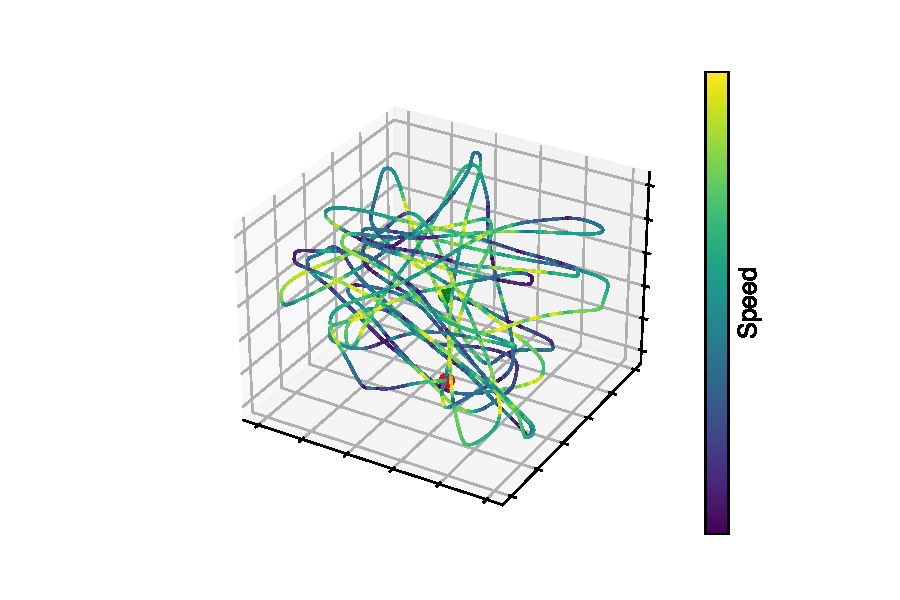
\includegraphics[width=1.0\textwidth,clip,trim={60 70 60 70}]{figures/bat_trajectory.pdf}
        \caption{}
        \label{subfig:trajectory}
    \end{subfigure}
    \\
    \vspace{0.5cm}
    \begin{subfigure}{0.32\textwidth}
        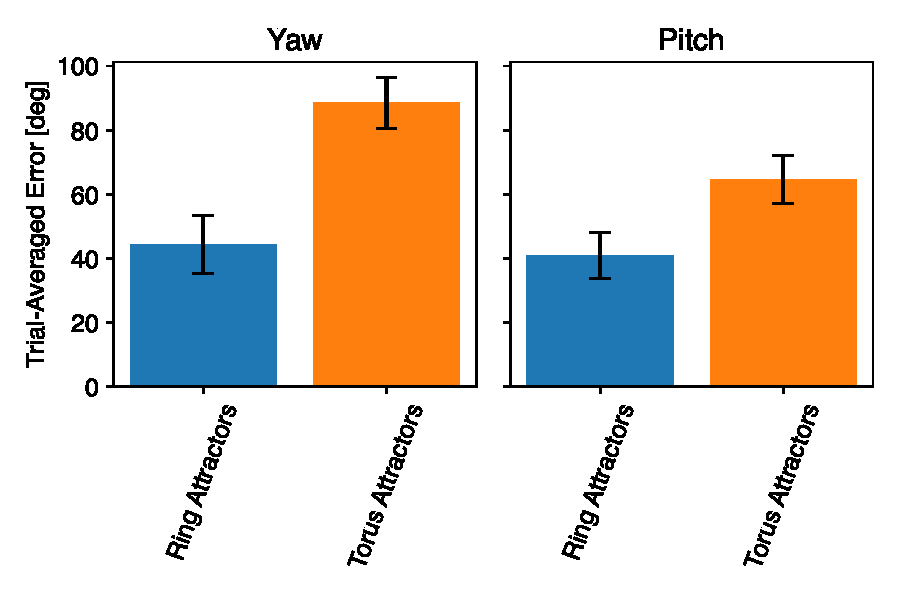
\includegraphics[width=1.0\textwidth]{figures/compare_full_torus/angular_error_comparison.pdf}
        \caption{}
        \label{subfig:torus_comparison}
    \end{subfigure}
    \begin{subfigure}{0.32\textwidth}
        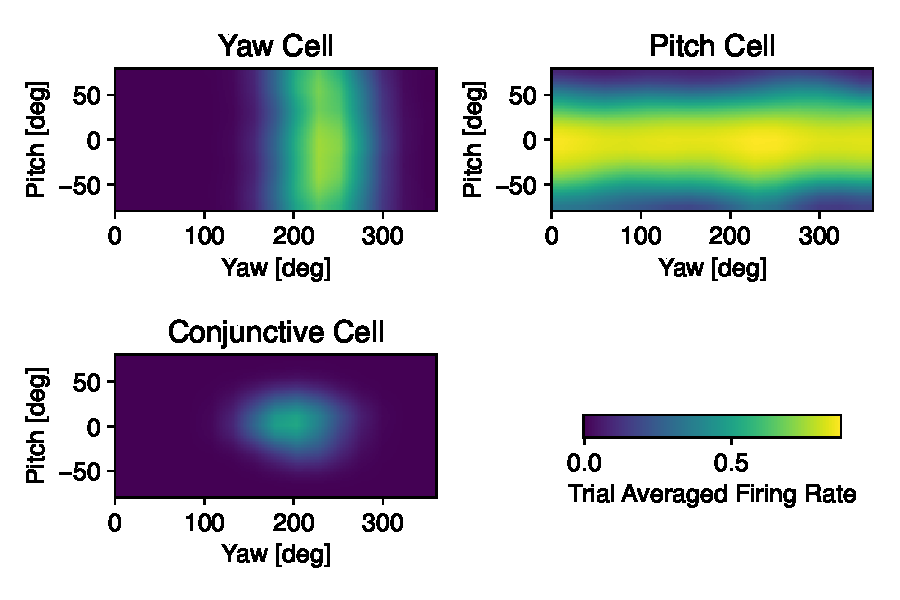
\includegraphics[width=1.0\textwidth]{figures/hebb_alt/bat_flight_cell_types_anchor.pdf}
        \caption{}
        \label{subfig:cell_types}
    \end{subfigure}
    \begin{subfigure}{0.32\textwidth}
        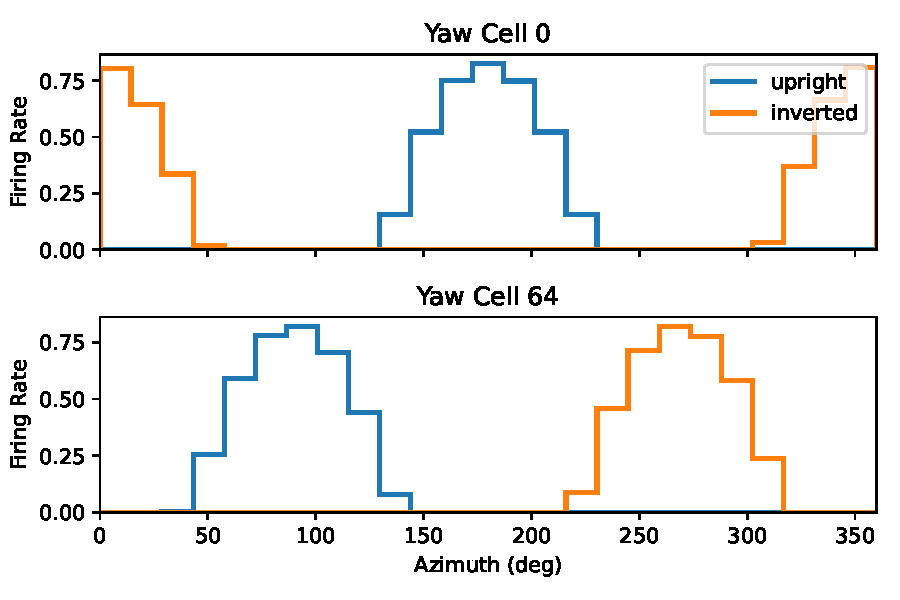
\includegraphics[width=1.0\textwidth]{figures/inverted_session/yaw_cells_activity_map.pdf}
        \caption{}
        \label{subfig:inversion}
    \end{subfigure}
    \\
    \vspace{0.5cm}
    \begin{subfigure}{0.65\textwidth}
        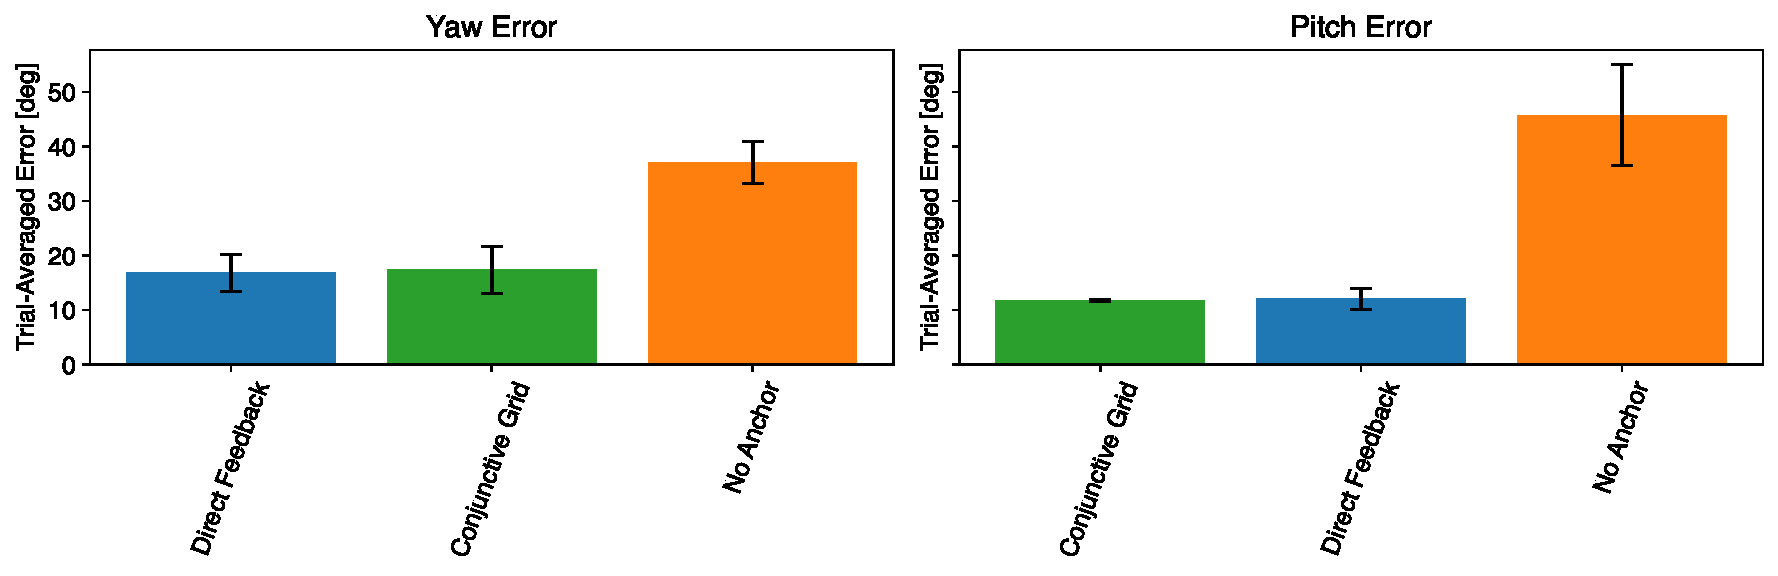
\includegraphics[width=1.0\textwidth]{figures/comparison/angular_error_comparison.pdf}
        \caption{}
        \label{subfig:drift_comparison}
    \end{subfigure}
    \begin{subfigure}{0.32\textwidth}
        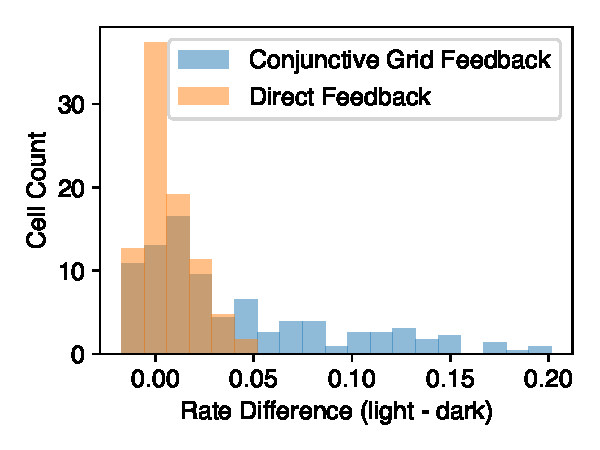
\includegraphics[width=1.0\textwidth]{figures/darkness/conj_cells_rate_difference_histogram.pdf}
        \caption{}
        \label{subfig:darkness_fire_rate}
    \end{subfigure}
    \caption{\subrefb{subfig:conj_feeback},~\subrefb{subfig:direct_feedback}~Schematics of the two circuit models. \subrefb{subfig:trajectory}~Example of a one-minute simulated bat flight. All simulated recordings below have a duration of $T=\SI{400}{\second}$. Both models use $N_{\text{yaw}}=256$ and $N_{\text{pitch}}=128$ neurons in the two rings, $N_{\text{landmark}}=40$ landmark cells, and a conjunctive population of $N_\text{conj}=20\times 10$ cells. \subrefb{subfig:torus_comparison}~Average drift over five trials without anchoring for the two-ring network and for a toroidal attractor of dimensions $N=256\times128$. \subrefb{subfig:cell_types}~Trial-averaged firing-rate maps of the different cell types as a function of yaw and pitch, obtained from the conjunctive-cell model with visual anchoring.
    \subrefb{subfig:inversion}~Trial-averaged firing rate of yaw-tuned cells as a function of the azimuth in upright and inverted posture, reproducing the inversion experiment of~\cite{Finkelstein2015}.
    \subrefb{subfig:drift_comparison}~Average drift of the two models compared to a model without anchoring (ten trials; error bars show the standard deviation across trials). \subrefb{subfig:darkness_fire_rate}~Difference in conjunctive-cell firing rate with and without visual input, for both models.}
    \label{figure}
\end{figure}
\newpage
\bibliography{literature.bib}
\end{document}

    % \begin{subfigure}{0.32\textwidth}
    %     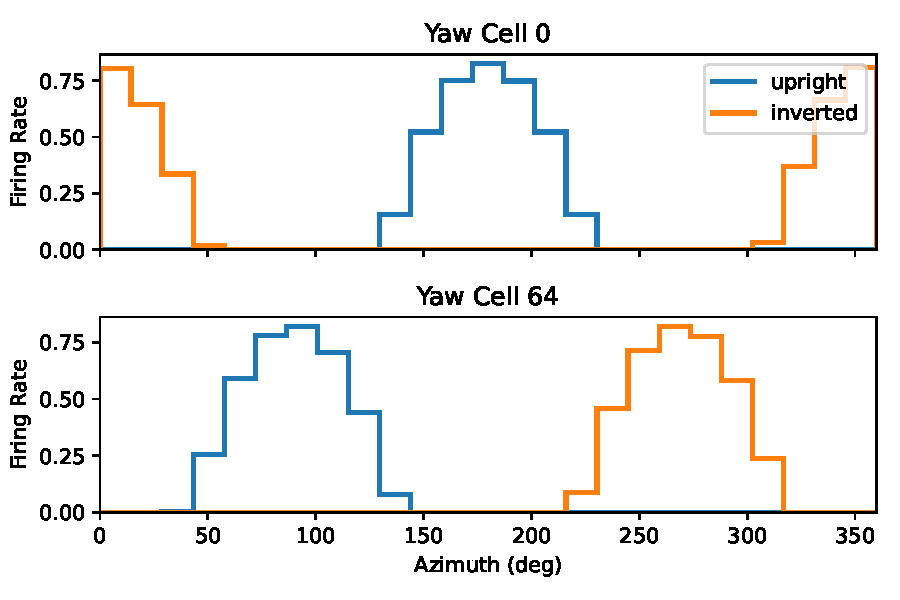
\includegraphics[width=1.0\textwidth]{figures/inverted_session/yaw_cells_activity_map.pdf}
    %     \caption{}
    %     \label{subfig:inversion}
    % \end{subfigure}